
\chapter{Strings in expanding universe}


In this chapter, we will discuss the motion of a~classical string in expanding universe \cite{zwiebach}. First, we assume that the metric has the form of the Friedmann-Lema\^{i}tre-Robertson-Walker (FLWR) metric

\begin{equation}
\label{eq:FLWR}
    \D s^2 = -\D t^2 + a(t)^2 \left[ \frac{\D r^2}{1-k r^2} + r^2 \lp \D \theta^2 + \sin^2 \theta \D \phi^2 \rp \right]
\end{equation}

\noindent
This metric describes a~homogeneous, isotropic and expanding universe with the ``scaling" of spatial coordinates $a(t)$. The constant $k \in \{-1, 0, +1\}$ represents the curvature of the space, but we will consider $k = 0$. When we solve the Einstein field equations, we get

\begin{align}
    &\lp \frac{\dot{a}}{a} \rp ^2 + \frac{k c^2}{a^2} = \frac{8 \pi G}{3} \rho \\
    2 \, \frac{\ddot{a}}{a} + & \lp \frac{\dot{a}}{a} \rp ^2 + \frac{k c^2}{a^2} = -\frac{8 \pi G}{c^2}P
\end{align}

\noindent
where $\rho$ is the total energy density, $P$ is pressure and $G$ is Newton's gravitational constant. Also, we will introduce the Hubble parameter of expansion of the universe as $H = \dot{a}/a$. The standard course of action would now be to consider contributions to the energy density $\rho$ and pressure $P$ from different sources, for example dust, radiation, cosmological constant. A~given proportion of these types of energy in the total energy density and pressure would give us the evolution of of this Hubble parameter $H$.

However, in our case we will consider the Hubble parameter $H$ to be constant. Currently, the latest measurement of the Hubble constant by the Fermi-LAT is $H = 68.0 \pm 4.2 ~ \rm{km s^{-1} Mpc^{-1}}$ \cite{hubble}. If the Hubble parameter is constant, then the metric in \cref{eq:FLWR} becomes

\begin{equation}
    \D s^2 = - \D t^2 + \me^{2Ht} \left[ \D r^2 + r^2 \lp \D \theta^2 + \sin^2{\theta}\D \phi^2 \rp \right]
\end{equation}

\noindent
For the motion of strings in this space, we will restrict ourselves to closed strings, that are always circular. The metric in cylindrical coordinates then takes the form

\begin{equation}
    \D s^2 = - \D t^2 + \me^{2Ht} \lp \D r^2 + r^2\D \theta^2 + \D z^2 \rp
\end{equation}

\noindent
A~natural parameterization for a~circular string is $\theta = \sigma$, while $r$ does not depend on $\sigma$, so $r = r\,(\tau)$. Also, because of the circularity of the string, we can rotate and translate the coordinate system such that $z = 0$. For the $\tau$ parameterization, we will choose the static gauge $t = \tau$. The vector of the string coordinates in the target space then takes the form

\begin{equation}
\label{eq:DSS_X}
    X^M = 
    \begin{pmatrix} 
    t = \tau, & r(\tau), & \theta = \sigma, & 0
    \end{pmatrix}.
\end{equation}

\noindent
The derivatives with respect to the world-sheet parameters are given by

\begin{align}
    \difs[] {X^M} {\tau} & = 
    \begin{pmatrix}
    1, & \dot{r}, & 0, & 0
    \end{pmatrix} \label{eq:DSS_x.}
    \\[8pt]
    \difs[] {X^M} {\sigma} & = 
    \begin{pmatrix} 
    0, & 0, & 1, & 0
    \end{pmatrix} \label{eq:DSS_x,}
\end{align}

\noindent
Since we have already chosen our parameterization, we will first calculate the action and use the Euler-Lagrange equations. This might look like too much simplification compared to the derivation in \cref{sec:general_EOM}, but we will show that we are allowed to use this approach in \cref{sec:desiter_general}.


%%%%%%%%%%%%%%%%%% SECTION %%%%%%%%%%%%%%%%%%%%%
\section{Lagrange approach}

In this section, we will look at the Lagrangian and try to find information about the system. Then, we will calculate the equations of motion and find the solutions.

\subsection{Lagrangian and potential}

We start with inserting \crefrange{eq:DSS_X}{eq:DSS_x,} into \cref{eq:action}

\begin{equation}
    \begin{aligned}
        S &= -T_0 \int\limits_{\tau_i}^{\tau_f} \D \tau \int\limits_{0}^{\sigma_1} \D \sigma 
        \sqrt{ - \lp -1 + \dot{r}^2 ~ \me^{2Ht} \rp \lp r^2 ~ \me^{2Ht} \rp}\\ 
        &= -T_0 \int\limits_{t_i}^{t_f} \D \tau \int\limits_{0}^{\sigma_1} \D \sigma ~
        \lp \abs{r ~ \me^{Ht}} \sqrt{1 - \dot{r}^2 ~ \me^{2Ht}} \rp
    \end{aligned}
\end{equation}

\noindent
Since the Lagrangian density, the term within the integral, does not depend on $\sigma$, we can integrate over it and receive only a~factor of $\sigma_1$. Because $\theta$ is $2 \pi$ periodic, the choice of the parameterization $\theta = \sigma$ infers that $\sigma_1 = 2 \pi$. Moreover, we will perform a~change of coordinates $R = r ~ \me^{Ht}$, which will lead to great simplification in calculation of the equations of motion. The action then becomes

\begin{equation}
\label{eq:action_de_sitter}
    S = - 2 \pi T_0 \int\limits_{t_i}^{t_f} \D \tau ~
    \abs{R} ~ \sqrt{1 - \lp \dot{R} - HR \rp^2}
\end{equation}

\noindent
Just from this Lagrangian we can extract a~lot of information about the solution. We can, for example, look at strings with constant $R$ and find the corresponding potential $V(R)$ from the Lagrangian \cite{zwiebach}

\begin{align}
    L (t, R, \dot{R} ) & = - 2 \pi T_0 ~ \abs{R} ~ \sqrt{1 - ( \dot{R} - HR )^2} \label{eq:desiter_lagrangian} \\[8pt]
    & \Downarrow \quad V \lp t, R \rp = -L \lp t, R, 0 \rp \nonumber \\[8pt]
    V(R) & = 2 \pi T_0 ~ \abs{R} ~ \sqrt{1 - ( HR )^2}
\end{align}
\vspace{0mm}


\noindent
This potential for static strings is plotted in \cref{fig:potential_de_sitter}. 

\begin{figure}[ht]
    \centering
    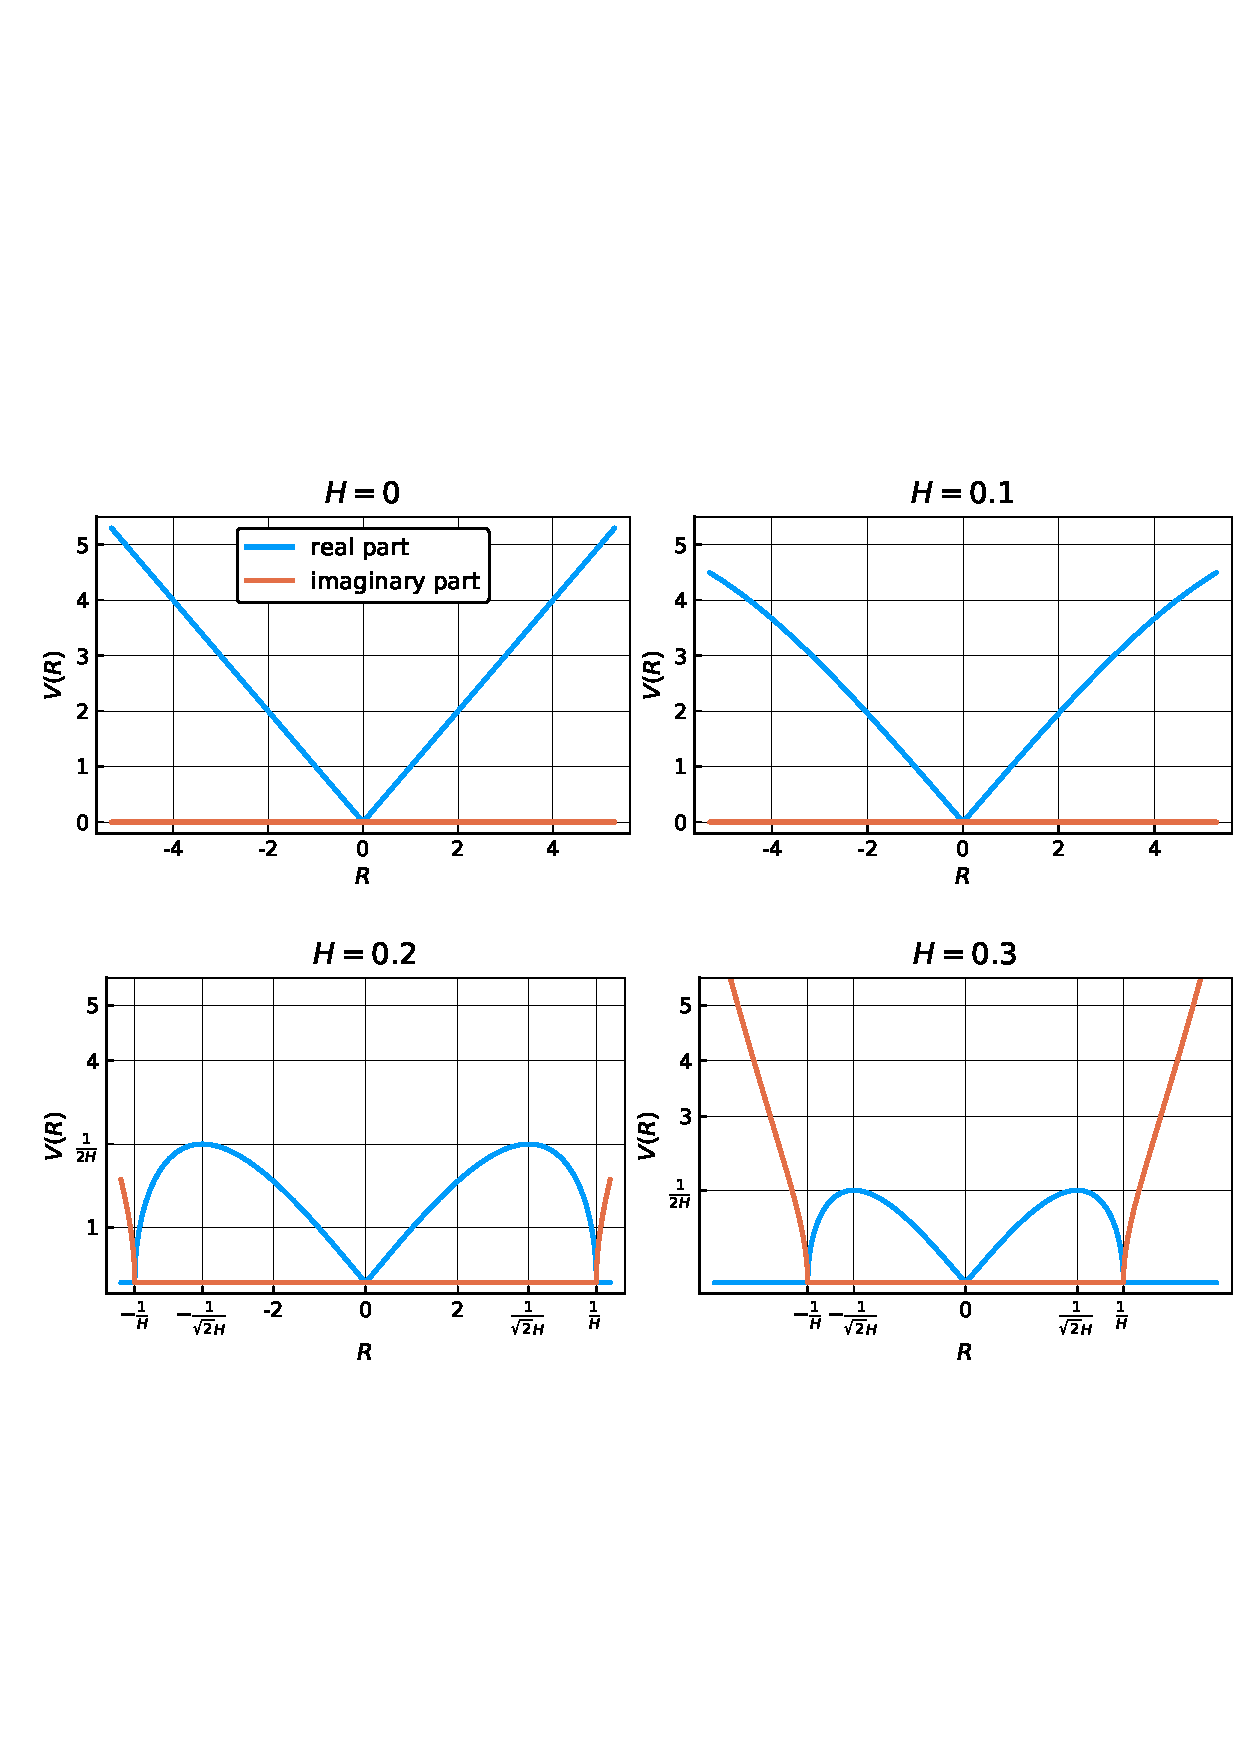
\includegraphics[width = 1.0\linewidth]{Pictures/potential.pdf}
    \caption{Potential for statics strings.}
    \label{fig:potential_de_sitter}
\end{figure}

We can immediately see, that the potential is well defined only for $R \leq 1/H$ and that there is a~potential well with minimum at $R = 0$ and maximum at $R = \pm 1/\sqrt{2} H$. This hints towards the fact, that every string that goes through the point $\dot{R} = 0, ~\abs{R} < 1/\sqrt{2} H$ will have a~closed trajectory in phase space. On the other hand, strings that pass through the point ($\dot{R} = 0, ~1/\sqrt{2} H < \abs{R} < 1/H $) expand infinitely or until they break.

%%%%%%%%%%%%%%%%%%% SUBSECTION %%%%%%%%%%%%%%%%%%%%%%%
\subsection{Equations of motion and critical points}
\label{sec:EOM_critpoints}

A~more complex analysis requires us to solve the equations of motion. The variation of action \eqref{eq:action_de_sitter} gives the same result as in classical mechanics, so we can use the Euler-Lagrange equations

\begin{equation}
    \dif[] {} {t} \lp \pardif[] {L} {\dot{R}} \rp - \pardif[] {L} {R} = 0
\end{equation}

\noindent
After some calculations, we will get the equations of motion in this form:

\begin{equation}
\label{eq:desiter_diff_eq}
    \frac{R \ddot{R} - \dot{R}^2 + 1 + 3HR \lp \dot{R} - HR \rp - 2HR \lp \dot{R} - HR \rp^3 }{\left[ 1 - \lp \dot{R} - HR \rp^2 \right]^{3/2}} = 0
\end{equation}

\noindent
We will split this differential equation of second order into two differential equations of first order by denoting $S = \dot{R}$. This leads to a~system of differential equations in the form:

\begin{equation}
\label{eq:system_EOM}
\begin{aligned}
        \dot{S} & = \frac{S^2 - 1 - 3HR \lp S - HR \rp + 2HR \lp S-HR \rp^3 }{R} \\
        \dot{R} & = S 
    \end{aligned}
\end{equation}

\noindent
We already mentioned, that there are four interesting points in the potential, namely $S = 0$ with $R = \pm  1/\sqrt{2}H$ and $R = \pm 1/H$. The former correspond to a~maximum of the potential, so these should be unstable nodes. But we cannot say much about the latter just from potential. However if we look at the equations of motion, these points can be studied in more detail. 

Let us first take a~look at the first one, $R = \pm 1/\sqrt{2}H$. Since the equations are symmetric around the origin, we can drop the $\pm$ sign and the results apply to both points. When we insert the values of $S$ and $R$, we get

\begin{equation}
     \begin{aligned}
        \dot{S} &= \left[ -1 - \frac{3}{\sqrt{2}} \lp -\frac{1}{\sqrt{2}} \rp + \frac{2}{\sqrt{2}} \lp \frac{1}{\sqrt{2}} \rp ^3  \right] \sqrt{2} H = \left[ -1 + \frac{3}{2} - \frac{1}{2} \right] \sqrt{2} H = 0 \\
        \dot{R} &= 0
     \end{aligned}
\end{equation}

\noindent
This is a~critical point in phase space, because the velocity vector field is zero at this point. For further study, we will linearize \cref{eq:system_EOM} in the neighborhood of this point with $\delta S$ and $\delta R$ being the distance from this point. We arrive at a~linear system of differential equations:

\begin{equation}
    \begin{pmatrix}
        \delta \dot{S} \\ \delta \dot{R}
    \end{pmatrix}
    =
    \bf{A} \cdot
    \begin{pmatrix}
        \delta S \\ \delta R
    \end{pmatrix} =
    \begin{pmatrix}
        a & b \\
        c & d
    \end{pmatrix}
    \begin{pmatrix}
        \delta S \\ \delta R
    \end{pmatrix},
\end{equation}

\noindent
where $A$ is a~matrix. 

If we calculate the eigenvalues and eigenvectors of $\bf{A}$, we can classify the critical points. There are three types of critical points depending on the eigenvalues: 
\begin{itemize}
    \item Both eigenvalues are positive $\implies$ unstable (repulsive) node -- all velocity vectors point away from the critical point
    \item Both eigenvalues are negative $\implies$ stable (attractive) node -- all velocity vectors point towards the critical point
    \item Eigenvalues are of opposite sign $\implies$ saddle -- eigenvectors divide regions of similar flow of velocity vector field
\end{itemize}

\noindent
In the case of the critical point at $R = 1/\sqrt{2}H$, we will first expand \cref{eq:system_EOM} in the neighbourhood such that $R = 1/\sqrt{2}H + \delta R$, $S =  0+ \delta S$ and then consider only the terms of the first order in both $\delta R$ and $ \delta S$ to be of significance. 
After some calculations we get:

\begin{equation}
    \begin{aligned}
        \delta \dot{S} & =  \frac{\delta S^2 - 1 - 3 \! \lp \! \frac{1}{\sqrt{2}} + \! H\delta R \rp \! \! \lp  \! \delta S - \! \frac{1}{\sqrt{2}} \! - H \delta R \rp \! + 2 \! \lp \! \frac{1}{\sqrt{2}} + \! H \delta R \rp  \! \! \lp \! \delta S - \! \frac{1}{\sqrt{2}} \! - H \delta R \rp^3}{\frac{1}{\sqrt{2} H} + \delta R} \\[0.3cm]
        & =  2H^2 \delta R + \mathcal{O}(\delta S^2, \delta R^2, \delta S \delta R)\\[0.3cm]
        \delta \dot{R} & = \delta S
    \end{aligned}
\end{equation}

\noindent
Rewritten into matrix equation

\begin{equation}
    \begin{pmatrix}
        \delta \dot{S} \\ \delta \dot{R}
    \end{pmatrix}
    =
    \begin{pmatrix}
        0 & 2H^2 \\
        1 & 0
    \end{pmatrix}
    \begin{pmatrix}
        \delta S \\ \delta R
    \end{pmatrix}.
\end{equation}

\noindent
From the characteristic equation, we arrive at the eigenvalues $\lambda$:

\begin{equation}
    \det 
    \begin{pmatrix}
        -\lambda & 2H^2 \\
        1 & -\lambda
    \end{pmatrix} = \lambda^2 - 2H^2 = 0, \qquad \lambda_{1,2} = \pm \sqrt{2} H
\end{equation}

\noindent
The eigenvalues are of opposite sign, which means, that we are looking at a~saddle point. Finding the eigenvectors will help us understand the flow of the vector field around the saddle point. Eigenvectors correspond to the direction in which the velocity has the same direction as the distance vector from the saddle point. So strings that are displaced from the critical point in the direction of the eigenvector will move steadily in that direction either inwards or outwards, depending on the associated eigenvalue.

\begin{align}
    \begin{pmatrix}
        \sqrt{2}H & 2H^2 \\
        1 & \sqrt{2}H
    \end{pmatrix} 
    \begin{pmatrix}
        a \\ b
    \end{pmatrix} 
    = \begin{pmatrix}
        0 \\ 0
    \end{pmatrix} \implies
    v_1 = \begin{pmatrix}
        -\sqrt{2}H \\ 1
    \end{pmatrix}
    \\
    \begin{pmatrix}
        -\sqrt{2}H & 2H^2 \\
        1 & -\sqrt{2}H
    \end{pmatrix} 
    \begin{pmatrix}
        c \\ d
    \end{pmatrix} 
    = \begin{pmatrix}
        0 \\ 0
    \end{pmatrix} \implies
    v_2 = \begin{pmatrix}
        \sqrt{2}H \\ 1
    \end{pmatrix}
\end{align}

\noindent
The eigenvectors and the flow of the velocity vector field are depicted in \cref{fig:eigvec_saddle}.

\begin{figure}[h]
    \centering
    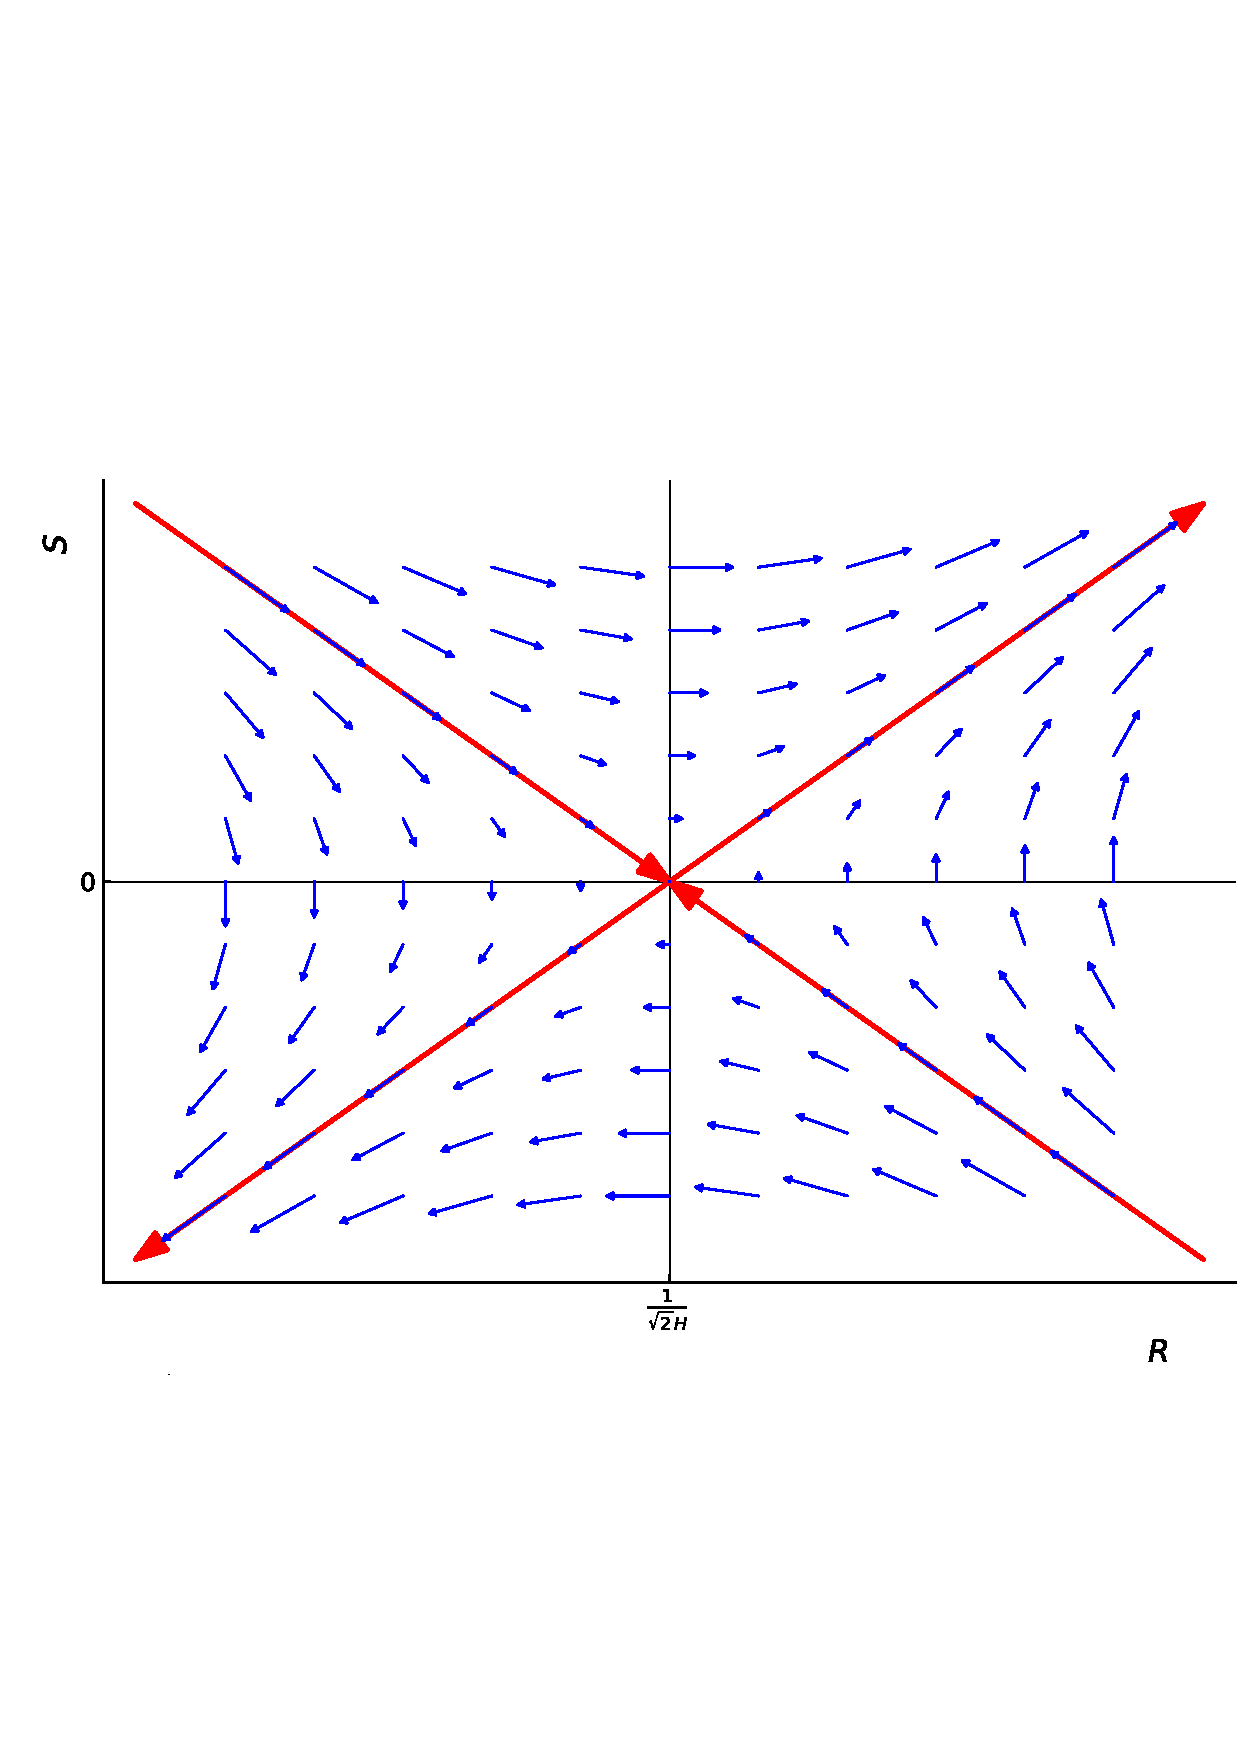
\includegraphics[width = 0.8\textwidth]{Pictures/saddle.pdf}
\caption{Eigenvectors (red) and flow of the velocity vector field (blue) around the saddle point $(R, S) = (1/\sqrt{2} H, 0)$.}
\label{fig:eigvec_saddle}
\end{figure}

%%%%%%%%%%%%%%%%%%%%%%%% REPULSIVE POINT %%%%%%%%%%%%%%%%%%%%%%%%%

We will now focus our attention on the second critical point at $S =0$, $R = \pm 1/H$. When we again look at the velocity vector field directly at this point, we get

\begin{equation}
    \dot{S} = \frac{-1 -3(-1) +2 (-1)^3}{\frac{1}{H}} = (3-1-2)H = 0
\end{equation}

\noindent
We can see, that this is another critical point and we will proceed with the same method as above, to determine the type of this critical point. Substituting into similar coordinates in the neighborhood of the point $S = \delta S$, $R = 1/H + \delta R$ and taking only the terms up to first order in $\delta S$ and $\delta R$, we get:

\begin{equation}
    \begin{aligned}
        \delta \dot{S} & =  \frac{\delta S^2 -1 -3 (1 + H\delta R) (\delta S - 1 - H \delta R) + 2 (1+H \delta R) (\delta S - 1 - H \delta R)^3}{\frac{1}{H} + \delta R} \\[0.3cm]
        & =  3 H \delta S - 2H^2 \delta R + \mathcal{O}(\delta S^2, \delta R^2, \delta S \delta R)\\[0.3cm]
        \delta \dot{R} & = \delta S
    \end{aligned}
\end{equation}

\noindent
In matrix notation, we arrive at:

\begin{equation}
    \begin{pmatrix}
        \delta \dot{S} \\ \delta \dot{R}
    \end{pmatrix} = 
    \begin{pmatrix}
        3H & -2H^2 \\
        1 & 0
    \end{pmatrix}
    \begin{pmatrix}
        \delta S \\ \delta R
    \end{pmatrix}
\end{equation}
\vspace{0mm}

\noindent 
Solving the characteristic equation for eigenvalues $\lambda$ then gives us:

\begin{equation}
    \det     
    \begin{pmatrix}
        3H - \lambda & -2H^2 \\
        1 & -\lambda
    \end{pmatrix} = 
    \lambda^2 - 3H \lambda + 2H^2, \qquad \lambda_{1,2} = \frac{3H \pm H}{2}
\end{equation}

\noindent
In conclusion, we have found a~repulsive point, because both eigenvalues are positive. All velocity vectors in this vector field aim out of this critical point as it is depicted in \cref{fig:eigvec_repulse}. Eigenvectors can, again, tell us more about the flow of the velocity vector field

\begin{align}
    \begin{pmatrix}
        2H & -2H^2 \\
        1 & -H
    \end{pmatrix} 
    \begin{pmatrix}
        a \\ b
    \end{pmatrix} 
    = \begin{pmatrix}
        0 \\ 0
    \end{pmatrix} \implies
    v_1 = \begin{pmatrix}
        H \\ 1
    \end{pmatrix}
    \\
    \begin{pmatrix}
        H & -2H^2 \\
        1 & -2H
    \end{pmatrix} 
    \begin{pmatrix}
        c \\ d
    \end{pmatrix} 
    = \begin{pmatrix}
        0 \\ 0
    \end{pmatrix} \implies
    v_2 = \begin{pmatrix}
        2H \\ 1
    \end{pmatrix}
\end{align}

\begin{figure}
    \centering
    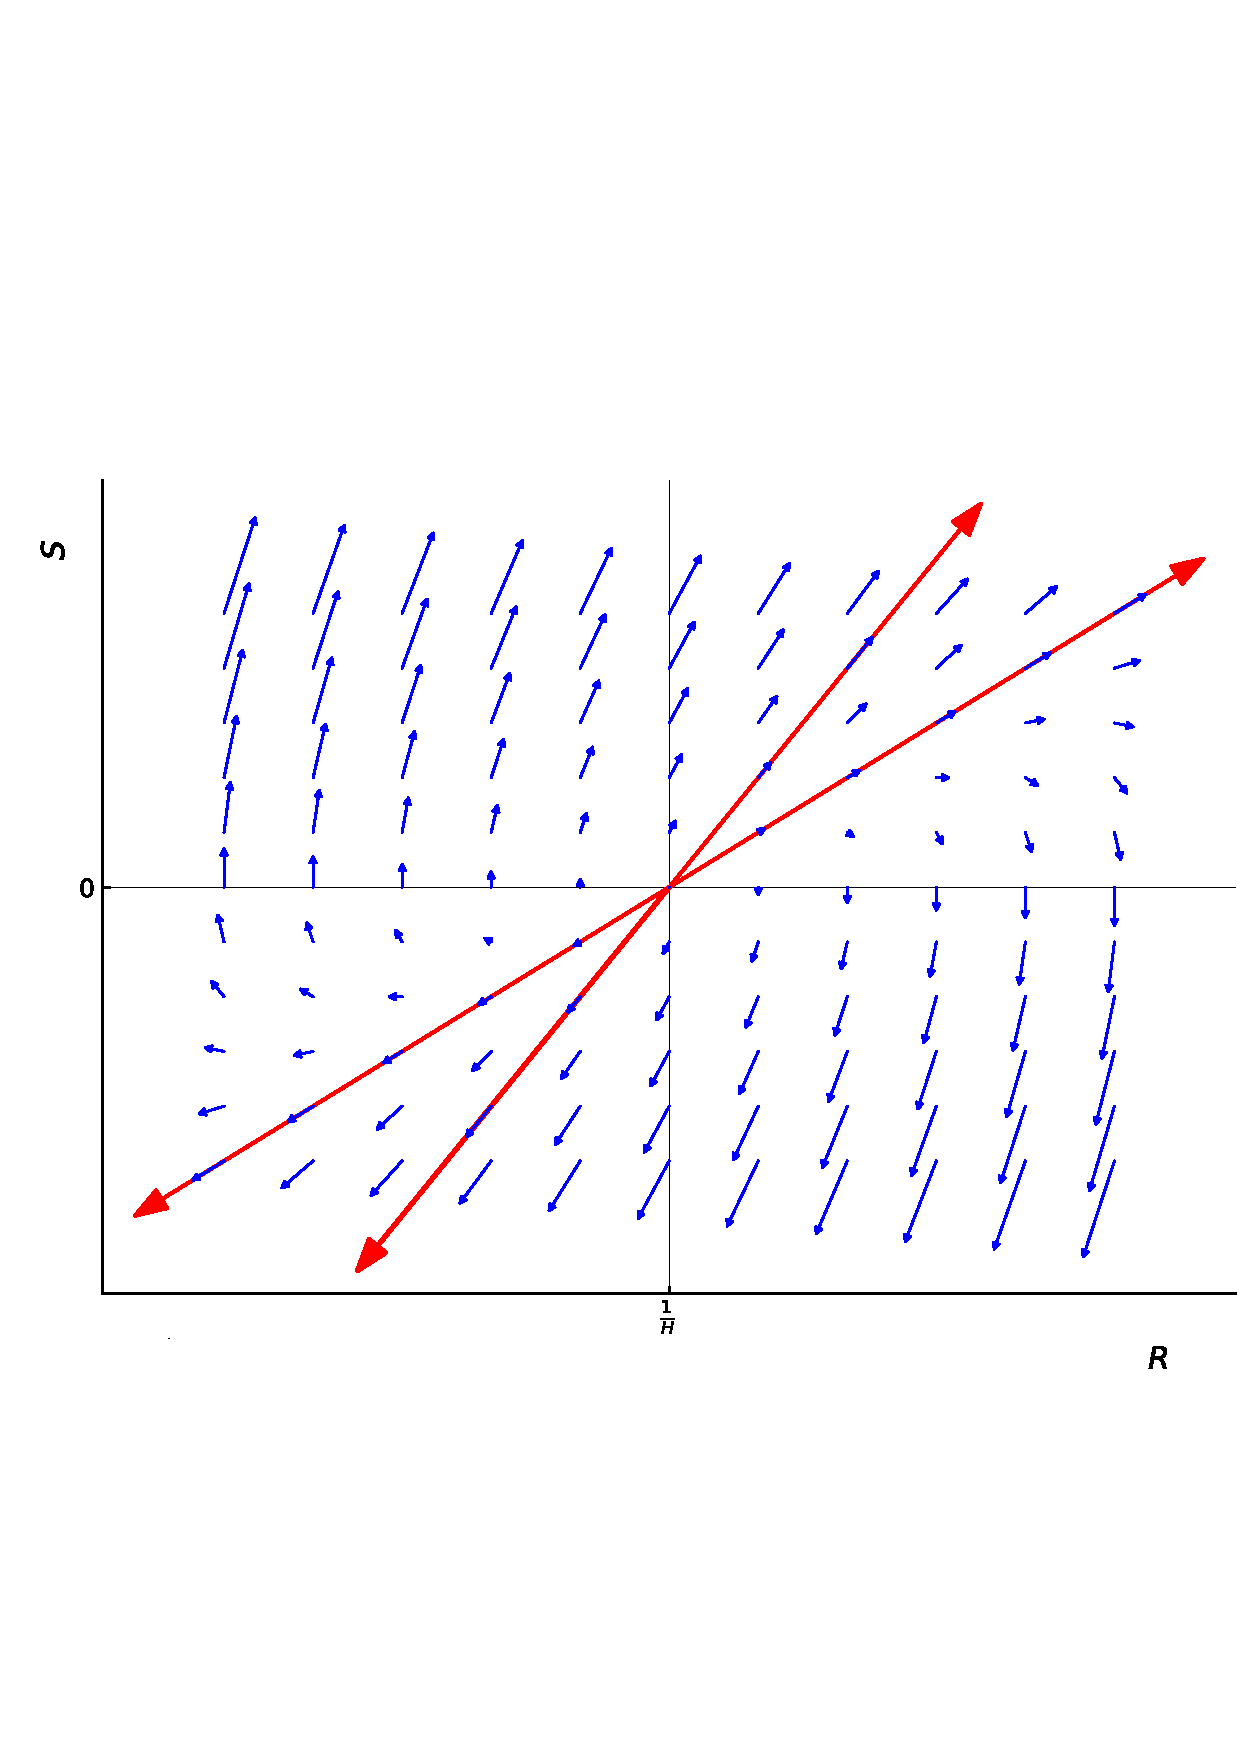
\includegraphics[width = 0.8\textwidth]{Pictures/unstable_node.pdf}
\caption{Eigenvectors (red) and flow of the velocity vector field (blue) around the unstable (repulsive) point (R, S) = (1/H, 0).}
\label{fig:eigvec_repulse}
\end{figure}

\noindent
These vectors are depicted in \cref{fig:eigvec_repulse} together with the flow of the velocity vector field.

Now, we would like to find explicit solutions. This gets a~little tricky, because we cannot solve these equations analytically, so we will proceed with finding numerical solutions. However, as it turns out, most trajectories pass through the axis $R = 0$. But at this point, the \cref{eq:system_EOM} contains a~singularity

\begin{equation}
    \lim\limits_{R \to 0} \dot{S} = \lim\limits_{R \to 0} \frac{S^2 - 1}{R} = \lim\limits_{R \to 0} \frac{(S - 1)(S + 1)}{R}
    \begin{cases}
        \pm \infty, & S \neq \pm 1 \\
        \frac{0}{0}, & S = \pm 1
    \end{cases}
\end{equation}

\noindent
In other words, $\dot{S}$ does not diverge only if $S$ goes to $\pm 1$ faster, than $R$ goes to $0$. If a~string passes through the $R = 0$ axis, it must do so at the speed of light $S = \pm 1$. As it turns out in the numerical solutions, this happens to be the case for every trajectory.

From this, however, arises another problem with this set of equations of motion. Even if $\dot{S}$ does not diverge, the numerical accuracy around this point has to be very high and almost unreachable for standard numerical solvers. We will therefore try to find a~different approach in which this singularity disappears and allows us to solve the equations with better numerical precision.



%%%%%%%%%%%%%%%%%%%%%%%%%%  SECTION  %%%%%%%%%%%%%%%%%%%%%%%%%%%%

\section{Conservation of energy}

As we can see in \cref{eq:desiter_lagrangian}, the Lagrangian does not depend explicitly on time $t$. This means, that the Hamiltonian and therefore the energy is conserved. We will denote the Hamiltonian as $\mathcal{E}$ to prevent ambiguity. Also, we will not perform the full Legendre transform, but we will express the Hamiltonian in terms of $\dot{R}$ and $R$

\begin{equation}
\label{eq:desiter_hamiltonian}
    \begin{aligned}
        \mathcal{E}(t, R, \dot{R}) = 2 \pi T_0 E(t, R, \dot{R}) = \pardif[] {L} {\dot{R}} \dot{R} - L(t, R, \dot{R}) & =  \\
        2 \pi T_0 \abs{R} \left[ \frac{\dot{R}^2 + \dot{R} HR}{\sqrt{1-(\dot{R}-HR)^2}} + \sqrt{1 - (\dot{R}-HR)^2}\right] & = 2 \pi T_0 \abs{R} \frac{1 + \dot{R}HR - H^2 R^2}{\sqrt{1-(\dot{R}-HR)^2}}
    \end{aligned}
\end{equation}


\noindent
where we used $\mathcal{E} = 2 \pi T_0 E$ to get a~more convenient form.
As we already mentioned, both the Lagrangian and Hamiltonian do not depend explicitly on time $t$ and therefore, the total energy $\mathcal{E}$ is conserved, $E = \text{const.}$ Furthermore, we will express $\dot{R}$ as a~function of $R$, $H$ and $E$. First, we square \cref{eq:desiter_hamiltonian} and then solve the quadratic equation for $\dot{R}$

\begin{equation}
\label{eq:desiter_S}
    S = \dot{R}(R, H, E) = \frac{\sqrt{E^2 + H^2 R^4 - R^2} \lp HR \sqrt{E^2 + H^2 R^4 - R^2} \pm E \rp}{E^2 + H^2 R^4}
\end{equation}

\noindent
where we denoted $S = \dot{R}$ as in previous section. This is much nicer function compared to \cref{eq:system_EOM}. First of all, it is a~first order differential equation. Second, there is no singularity at $R = 0$, and third, the critical points remain (as they should).

\subsection{Domain of definition}

Because of the square root in \cref{eq:desiter_S} and the fact that we do not want to expand our solutions to the complex plane, we can expect some conditions to arise for the domain of definition. These will arise from the condition that

\begin{equation}
\label{eq:desiter_sqrt_cond}
    E^2 + H^2 R^4 - R^2 \geq 0
\end{equation}

\noindent
For a~fixed and positive $H$ and $E$, we are going to look when this expression is satisfied. First, we look for the roots in $R$. 

\begin{equation}
\label{eq:desiter_sqrt_cond_R}
    R^2 = \frac{1 \pm \sqrt{1-4 E^2 H^2 }}{2H^2}
\end{equation}

\noindent
We can sort the condition into two cases. In the first case, we have $E>1/2H$. For this energy, there is no real value of $R$, for which the expression in \cref{eq:desiter_sqrt_cond} is equal to zero. That means that for such values of $E$, this condition is either always or never satisfied. Inserting any value larger, for example $E = 1/H > 1/2H$ and $R = 1/H$, we get

\begin{equation*}
    \frac{1}{H^2} + \frac{1}{H^2} - \frac{1}{H^2} = \frac{1}{H^2} > 0
\end{equation*}

\noindent
This is great, because the conditions is satisfied for every $R \in \Rbb$. In other words, the string can have any radius $R$ in the interval $\{-\infty, \infty\}$. 

On the other hand, if we look at energies $E < 1/2H$, we get two roots for $R^2$ and four roots for $R$. This splits $R$ into five regions that are separated by the roots of \cref{eq:desiter_sqrt_cond_R}. These regions are depicted in \cref{fig:intervals}, where we denote

\begin{equation}
\label{eq:desiter_r0}
    \begin{aligned}
    R^{+} = \sqrt{\frac{1 + \sqrt{1 - 4 E^2 H^2}}{2H^2}} \\
    R^{-} = \sqrt{\frac{1 - \sqrt{1 - 4 E^2 H^2}}{2H^2}}
    \end{aligned}
\end{equation}

\begin{figure}
\centering
\begin{tikzpicture}

\draw[thick,->] (-5.5,0) -- (5.5,0) node[anchor=north west] {R};
\draw[thick,->] (0,-1.5) -- (0,1.5) node[anchor=south east] {S};

\def\y{4}

\draw[ultra thick, red, ->] ($\y*sqrt(3)/2*(1,0)$) -- (5.5,0);

\draw[ultra thick, green] ($\y*1/2*(1,0)$) -- ($\y*sqrt(3)/2*(1,0)$);

\draw[ultra thick, blue] ($\y*1/2*(-1,0)$) -- ($\y*1/2*(1,0)$);

\draw[ultra thick, green] ($\y*sqrt(3)/2*(-1,0)$) -- ($\y*1/2*(-1,0)$);

\draw[ultra thick, red, <-] (-5.5,0) -- ($\y*sqrt(3)/2*(-1,0)$);

\filldraw [black] ($\y*sqrt(3)/2*(1,0)$) circle (3pt) node[anchor=north, black] {$R^{+}$};

\filldraw [black] ($\y*1/2*(1,0)$) circle (3pt) node[anchor=north, black] {$R^{-}$};

\filldraw [black] ($\y*1/2*(-1,0)$) circle (3pt) node[anchor=north, black] {$-R^{-}$};

\filldraw [black] ($\y*sqrt(3)/2*(-1,0)$) circle (3pt) node[anchor=north, black] {$-R^{+}$};

\end{tikzpicture}

\caption{Highlighted regions on $R$ axis, that are split by the roots of \cref{eq:desiter_sqrt_cond}.}
\label{fig:intervals}
\end{figure}


\noindent
Each of these regions must be examined separately, but we can still see the symmetry around $R = 0$, so we will only need to examine three of them. As is shown in \cref{fig:intervals}, we can group the intervals $R \in [-\infty, -R^{+}]$ and $R \in [R^{+}, \infty]$ as the red segments, and the intervals $R \in [-R^{+},-R^{-}]$ and $R \in [R^{-},R^{+}]$ as the the green segments. To find out where the condition \cref{eq:desiter_sqrt_cond} is satisfied, we need to evaluate it in every region. Let us start with the red interval $R \in [R^{+}, \infty]$:

\begin{equation}
    R = \frac{2}{H} > R^{+} \implies E^2 + \frac{16}{H^2} - \frac{4}{H^2} = E^2 + \frac{12}{H^2} > 0
\end{equation}

\noindent
In this region, strings with any energy can exist. Analogously for the green interval $R \in [R^{-},R^{+}]$:

\begin{equation}
    R^{+} > R = \frac{1}{\sqrt{2}H} > R^{-} \implies E^2 + \frac{1}{4 H^2} - \frac{1}{2 H^2} = E^2 -\frac{1}{4 H^2} < 0
\end{equation}

\noindent
The last inequality follows from the fact, that we are considering only $E < 1/2H$. Strings with such energy cannot exist in the green intervals.

The final interval is the blue interval $R \in [-R^{-}, R^{-}]$:

\begin{equation}
    R^{-} > R = 0 > -R^{-} \implies E^2 > 0
\end{equation}

\noindent
Again, this is a~region, where strings with all energies can exist.

In conclusion, we have two types of strings. First, we have strings with energy $E > 1/2H$ that have the domain of definition all of $R \in \Rbb$. Second, strings with energy $E < 1/2H$ have limitations. They can only exist in the red and blue regions depicted in \cref{fig:intervals}. We avoided the string with energy exactly $E = 1/2H$ for which the green regions vanish. This is not unexpected, because this string goes through the saddle point $S = 0$, $R =1/\sqrt{2}H$.

All this can also be interpreted physically from the potential in \cref{fig:potential_de_sitter}.
There we have a~potential well centered around $R = 0$ with maximum at $R = \pm 1/\sqrt{2}H$ and the corresponding value $V = 1/2H$. This implies that strings with energy lower than the maximum of this potential ($E < 1/2H$) are stuck inside this potential well. On the other hand if this string finds itself already outside of the potential well, it will expand to infinity. The strings that have energy above the potential barrier ($E > 1/2H$) can move over and therefore will never have closed solutions.


%%%%%%%%%%%%%%%%%%%%%%%%%%%%% SECTION %%%%%%%%%%%%%%%%%%%%%%%%%%%%%%

\section{Summary of results}

This brings us to the conclusion where we will present the phase space plots of the numerical solutions. First, we start with closed trajectories depicted in \cref{fig:desiter_closed}. These can happen only for strings with $E<1/2H$ and they are also the most likely to be observed, because of the fact, that our universe's expansion rate $H$ is relatively small, and we would need strings with very high energies to overcome the potential well. Strings that are not of cosmological magnitude therefore do experience little change. In \cref{fig:desiter_time_depend} we show the explicit time dependence of radius $R$ on time, which was acquired by numerical integration of \cref{eq:desiter_S}. If we compare it to the flat spacetime, where it is a~sine function, we can confirm, that for smaller energies, the expansion of space has little effect, but with increasing energy the trajectory gets more deformed and has increased frequency. 


On the other hand, the existence of the expansion of the universe can have some unforeseen consequences. It is surprising, that even with a~really small expansion rate, there can exist a~string with much larger radius than its counterpart stuck in closed trajectory. In fact, even a~string with $E = 0$ can have very large radius. This is due to the repulsive node in $R = 1/H$, where a~string with any energy can be created and then expand to infinity. This is shown in \cref{fig:desiter_closed_plus_expanding}.


This brings us to the special case where $E = 1/2H$. This is depicted as the purple line in \cref{fig:desiter_labile}. It would seem that when this string arrives at $R = 1/\sqrt{2}H$, it can decide whether to continue to the closed trajectory part or expand to infinity. However this dilemma solves itself, because it would take the string an infinite amount of proper time to reach this saddle point. 


The last case are strings with $E > 1/2H$ which is depicted in \cref{fig:desiter_unstable}. These strings can start as static strings at $R =1/H$, which is an unstable node. If these strings are then shifted by a~small amount, they either start to shrink, reach a~minimal radius and then expand or they expand to infinity right away.

All these solutions are constrained by the black lines and fill the whole of this space. For comparison, we add solutions in flat spacetime, that are depicted in \cref{fig:flat_closed}.

\begin{figure}[h]
    \centering
    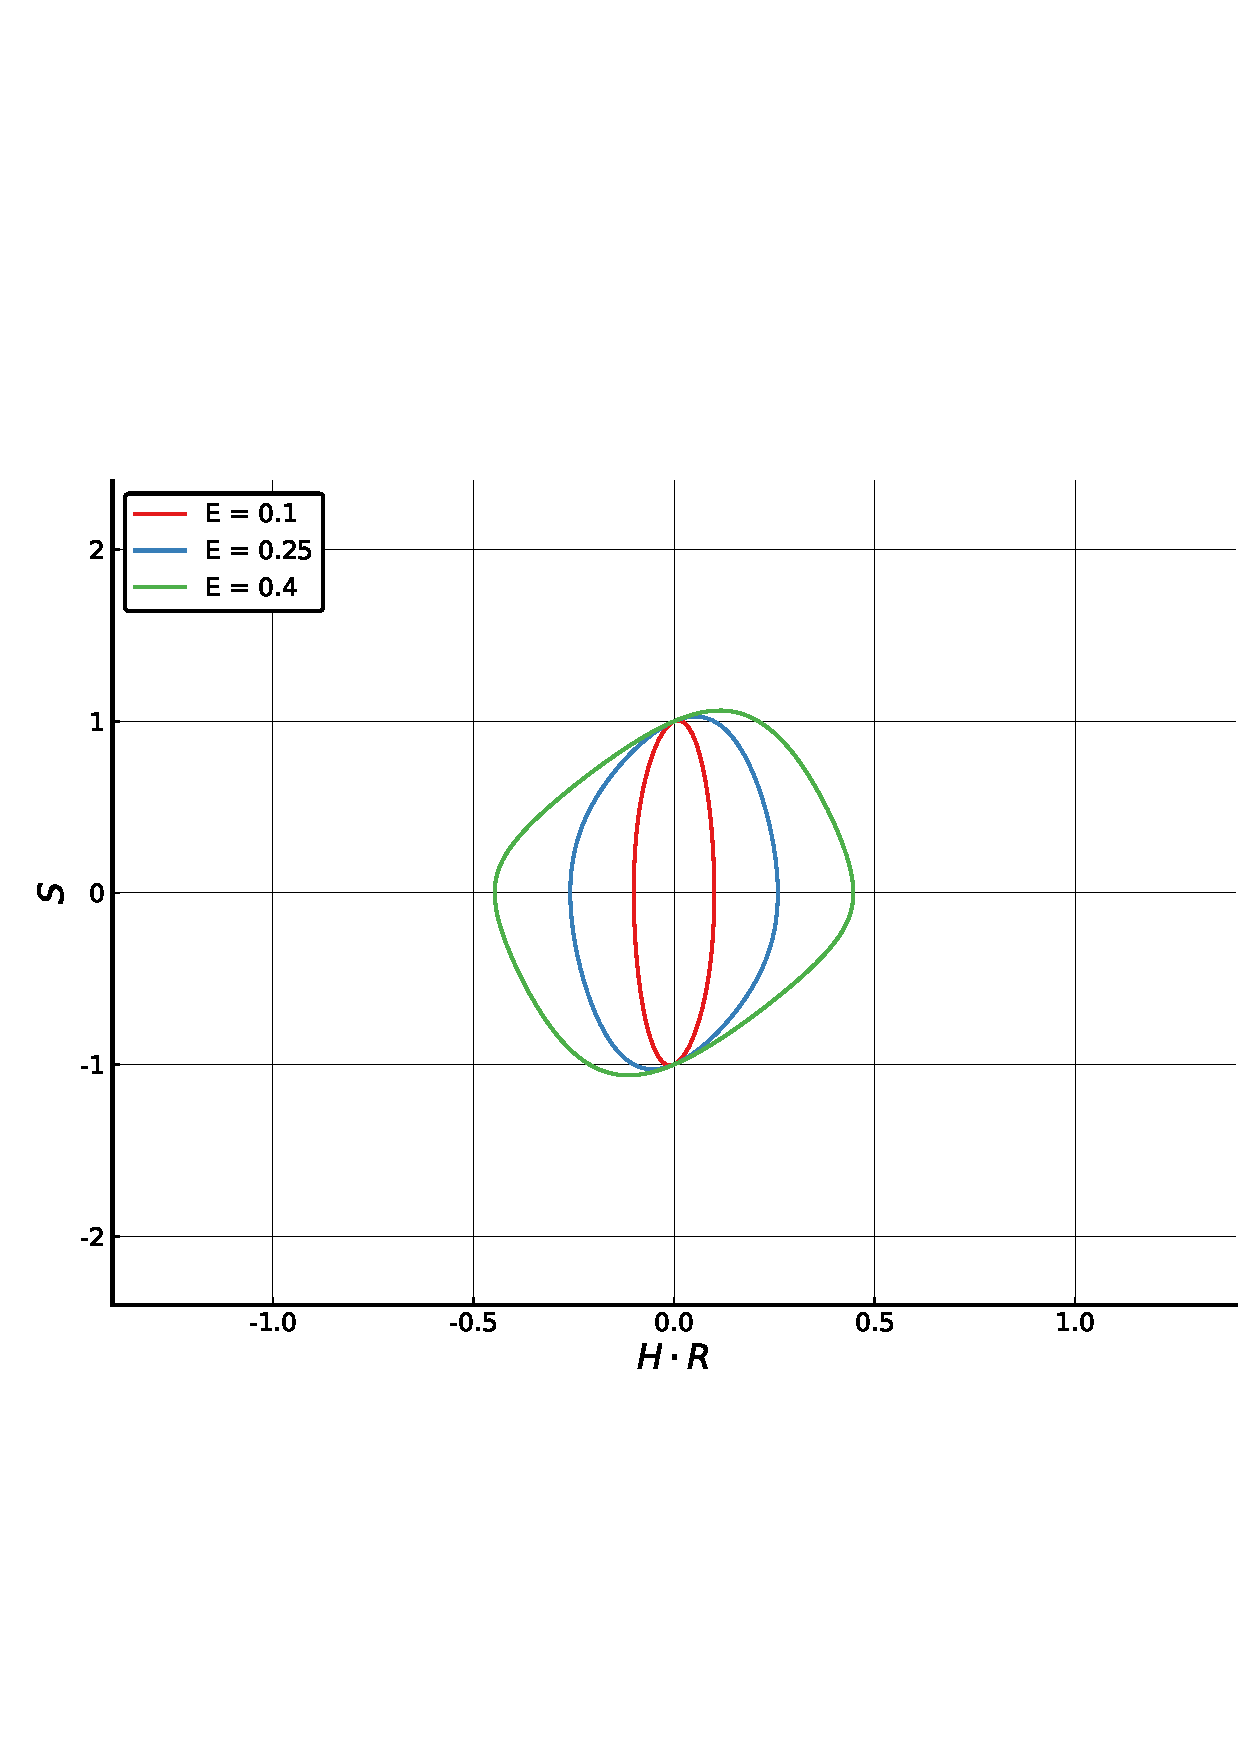
\includegraphics[width = 0.93 \linewidth]{Pictures/DeSitter_closed.pdf}
    \caption{Closed trajectories in de Sitter space for $E<1/2H$.}
    \label{fig:desiter_closed}
\end{figure}

\begin{figure}
    \centering
    \includegraphics[width = 0.93 \linewidth]{Pictures/DeSitter_closed_plus_expanding.pdf}
    \caption{All trajectories in de Sitter space for $E<1/2H$.}
    \label{fig:desiter_closed_plus_expanding}
\end{figure}

\begin{figure}
    \centering
    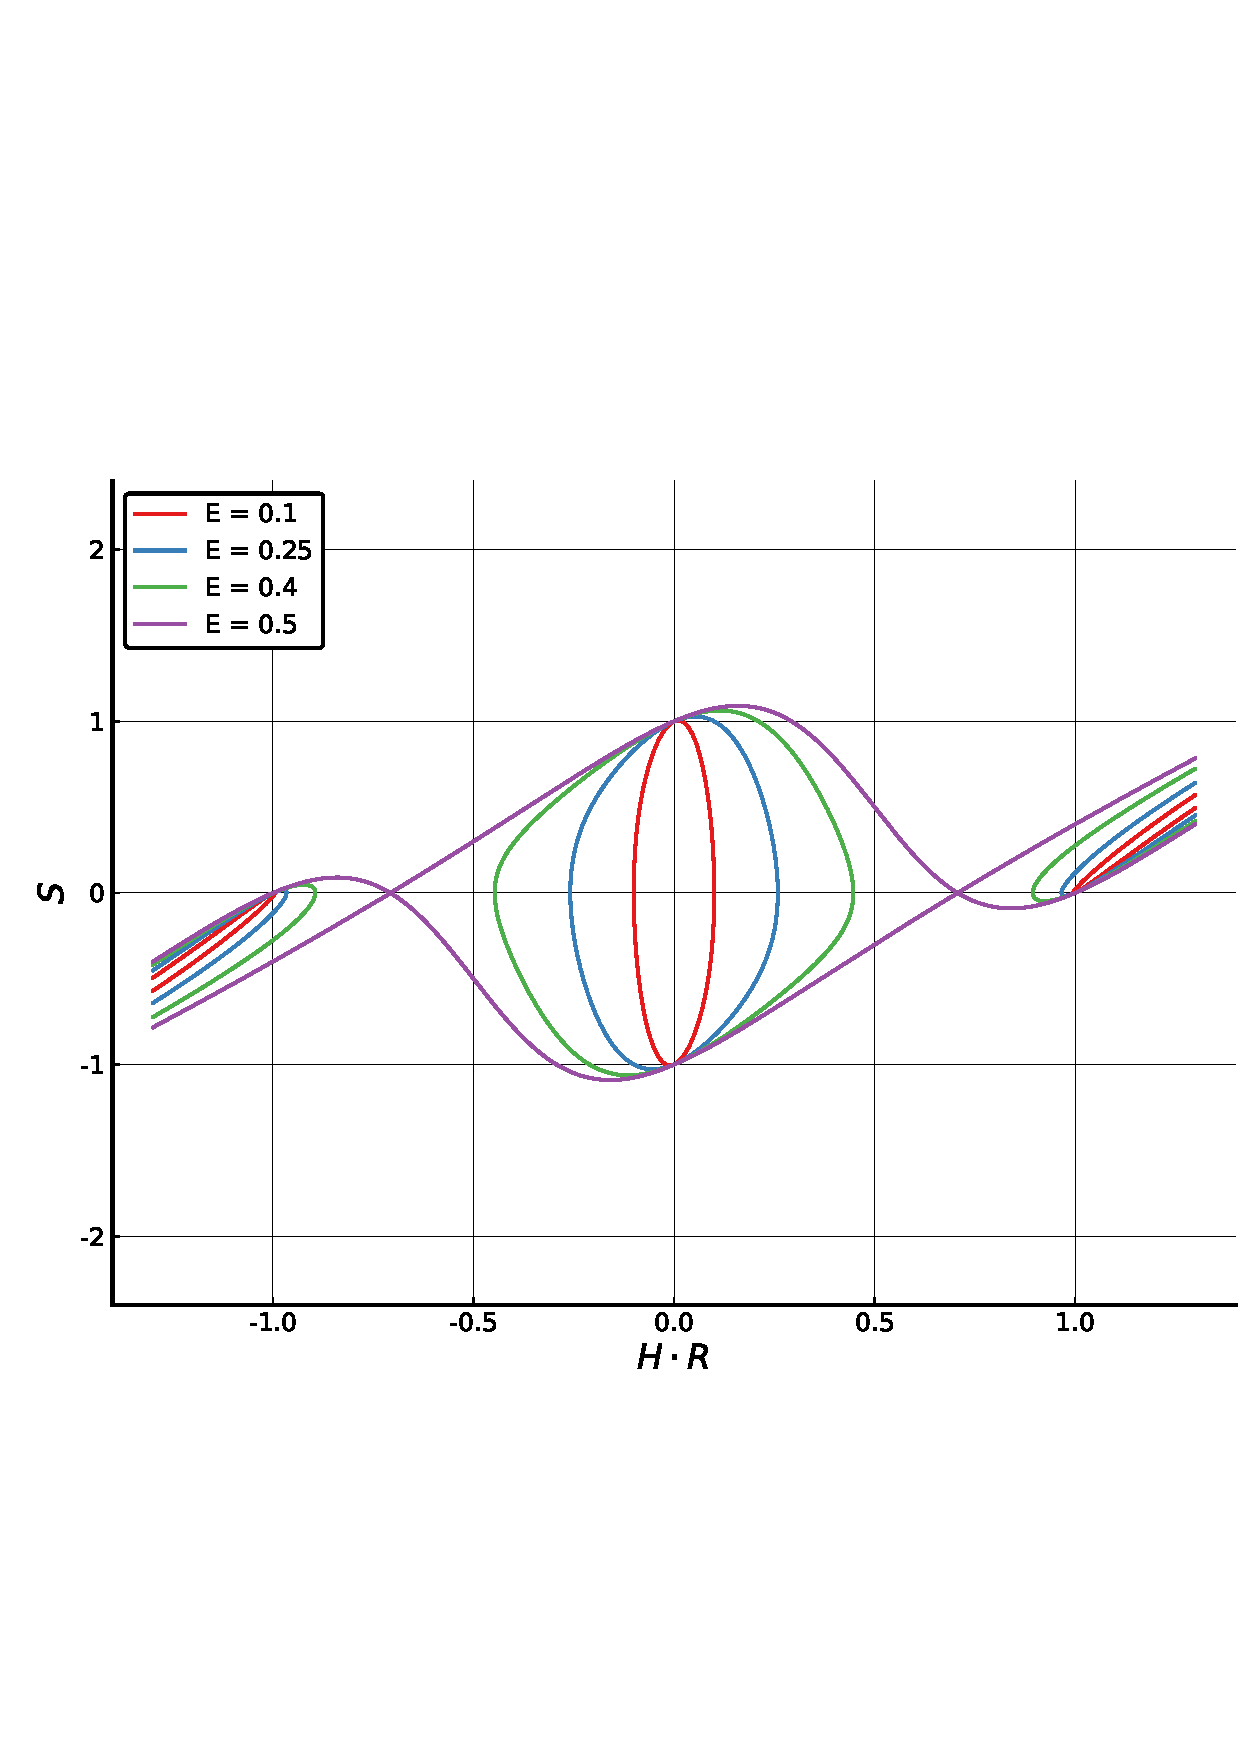
\includegraphics[width = 0.93 \linewidth]{Pictures/DeSitter_labile.pdf}
    \caption{All trajectories in de Sitter space for $E \leq 1/2H$.}
    \label{fig:desiter_labile}
\end{figure}

\begin{figure}
    \centering
    \includegraphics[width = 0.93 \linewidth]{Pictures/DeSitter_unstable.pdf}
    \caption{Trajectories for all energies $E$ in de Sitter space.}
    \label{fig:desiter_unstable}
\end{figure}

\begin{figure}
    \centering
    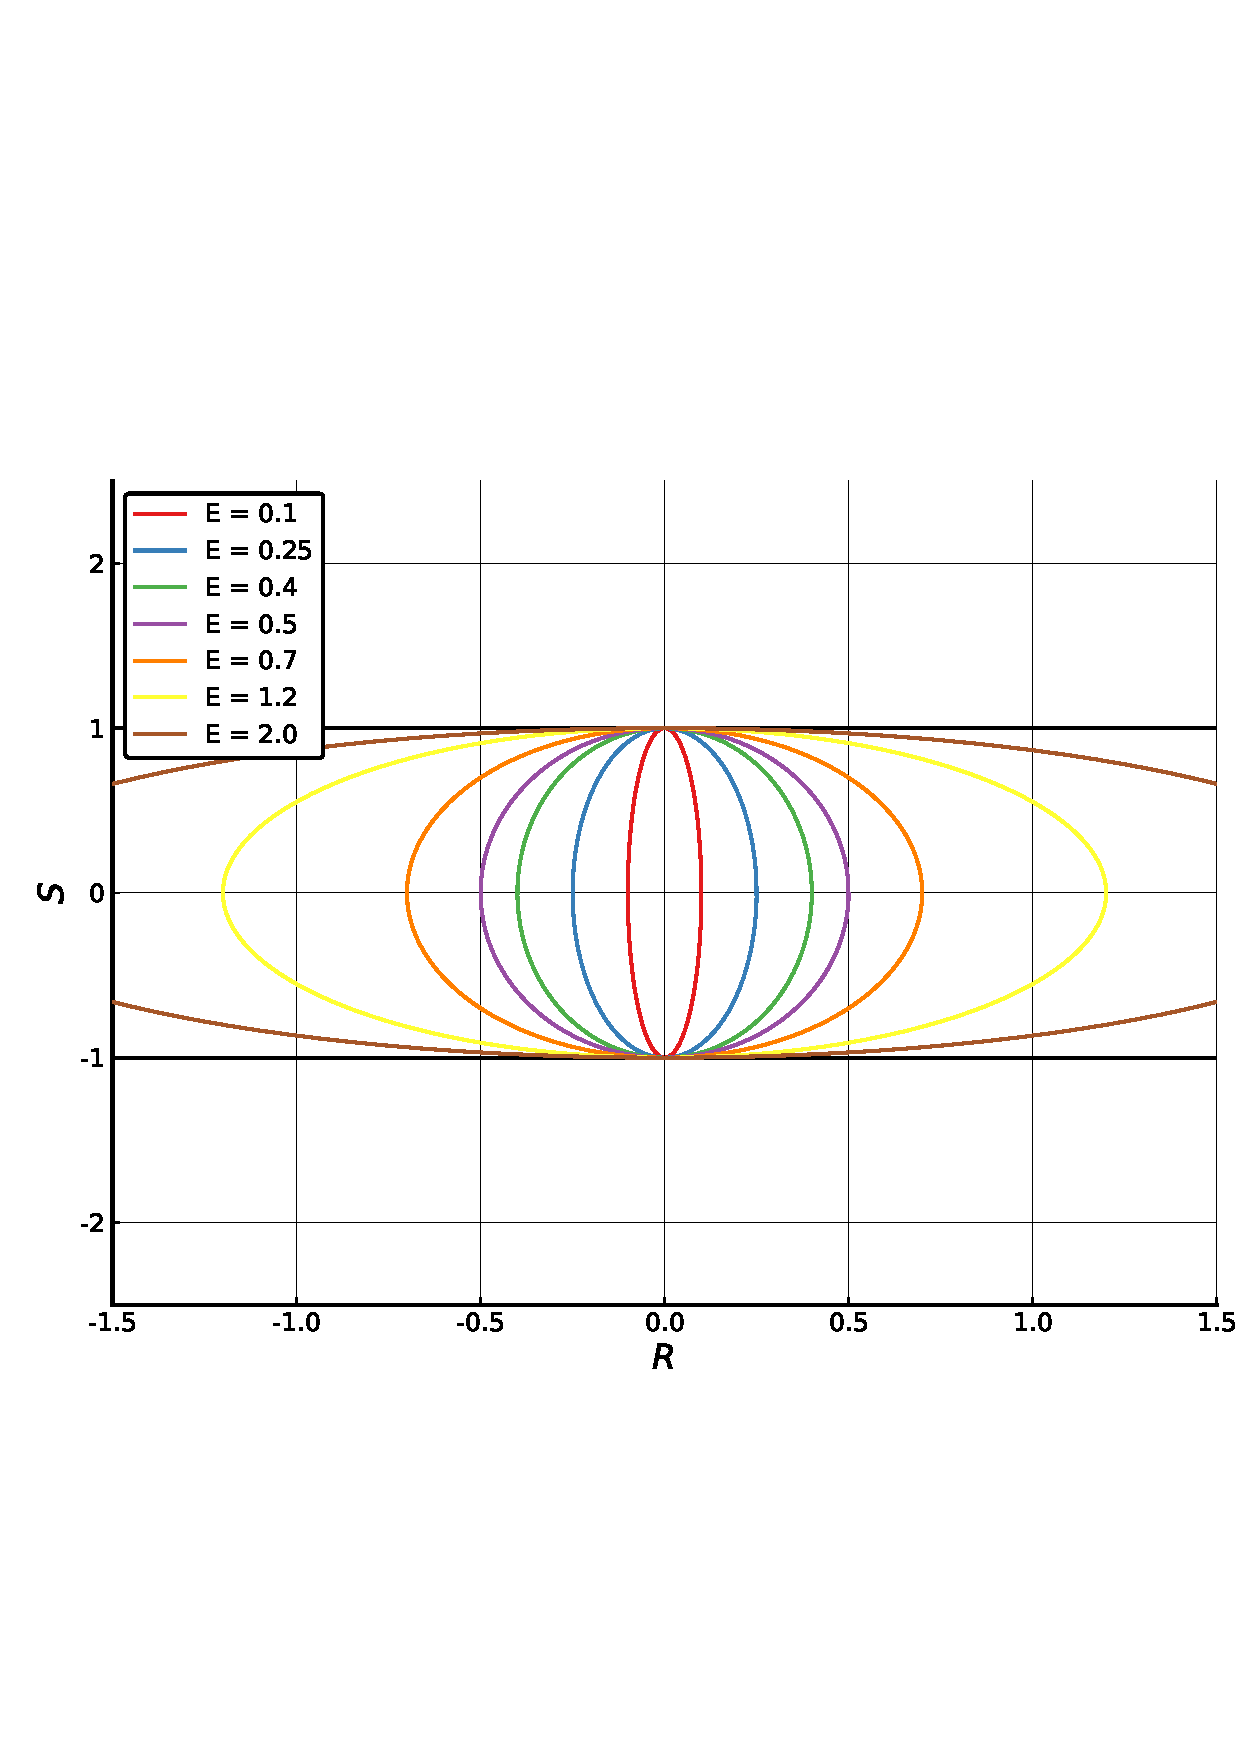
\includegraphics[width = 0.93 \linewidth]{Pictures/Flat_closed.pdf}
    \caption{Trajectories for all energies $E$ in flat space.}
    \label{fig:flat_closed}
\end{figure}

\begin{figure}
    \centering
    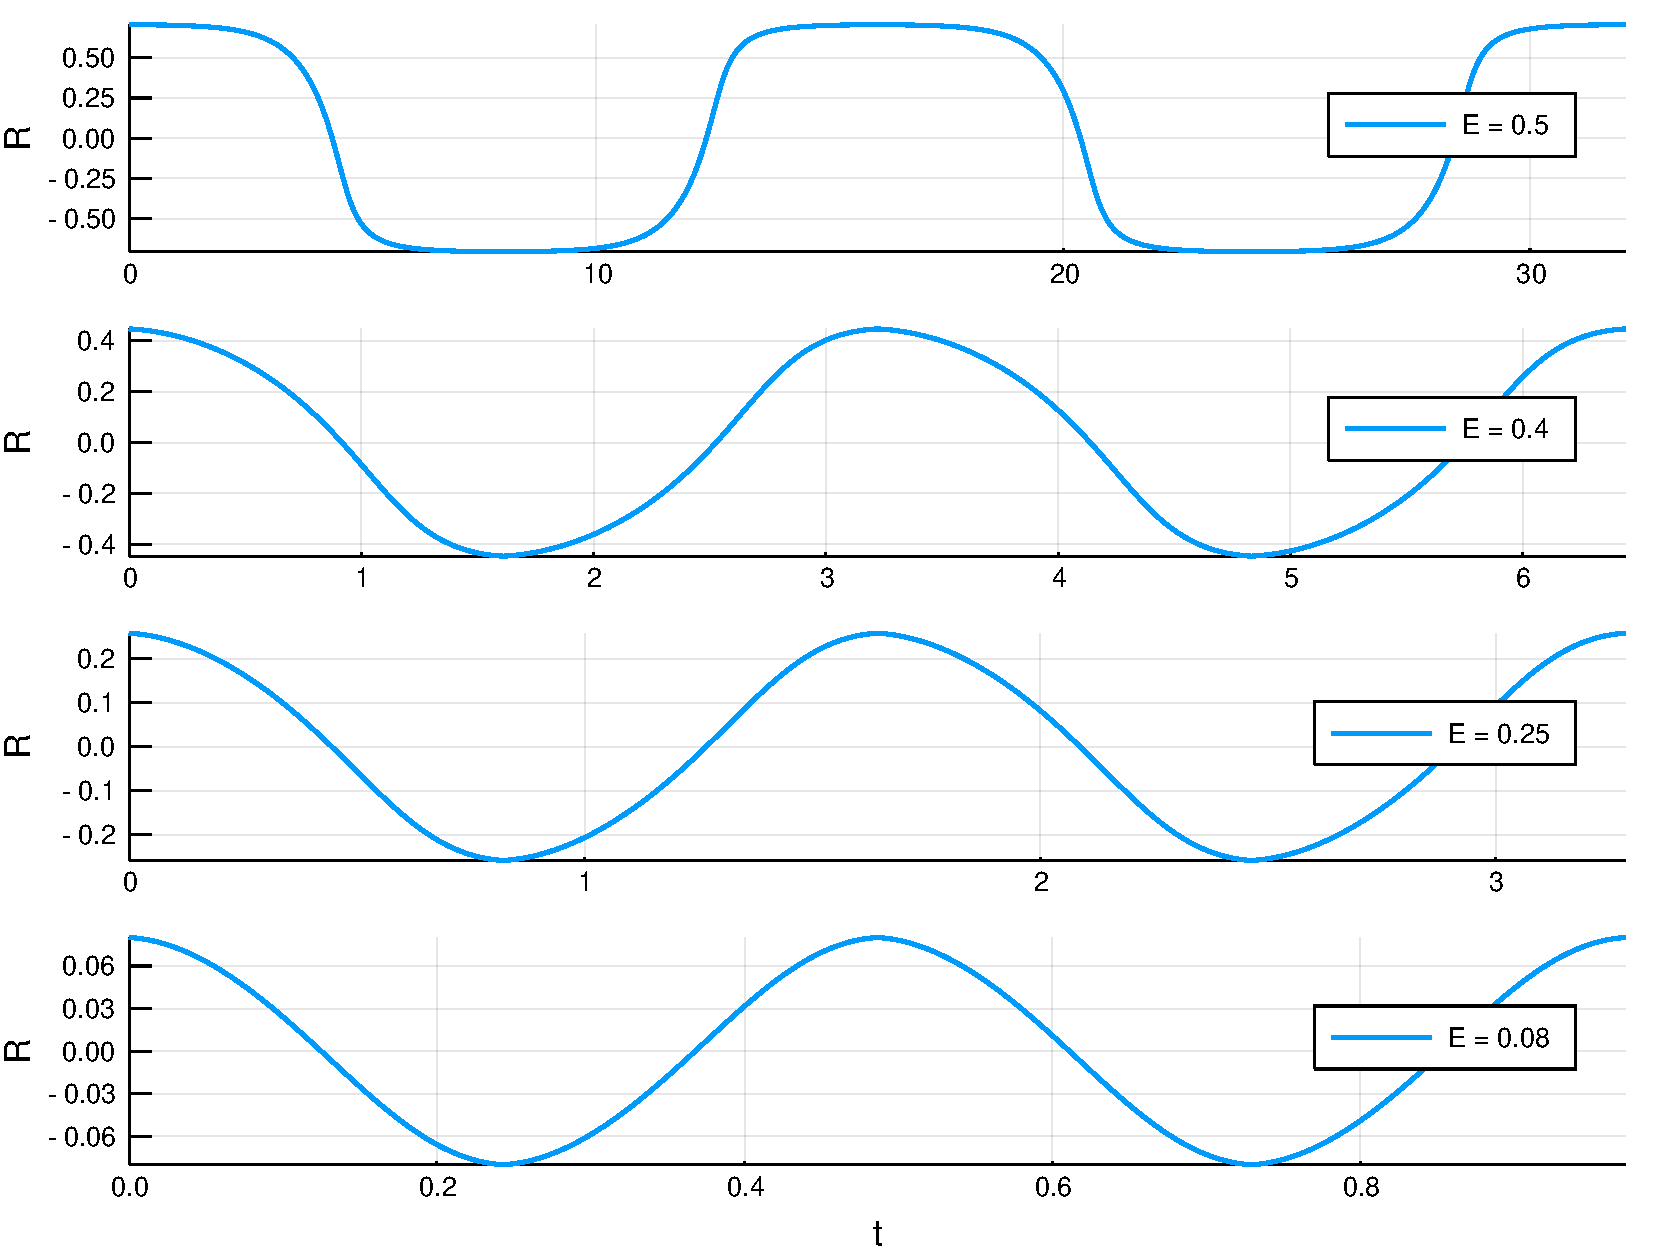
\includegraphics[width = 1.0 \linewidth]{Pictures/Time_dep.pdf}
    \caption{Explicit time evolution of closed strings with energies $E < 1/2H$}
    \label{fig:desiter_time_depend}
\end{figure}

%%%%%%%%%%%%%%%%%%%%%%%%%% SECTION %%%%%%%%%%%%%%%%%%%%%%%%%%%
\clearpage

\section{Verification with general equations of motion}
\label{sec:desiter_general}

In the beginning of this chapter we started with the Nambu--Goto action, and we immediately fixed the parameterization to $t = \tau$ and $\theta = \sigma$ and inserted a~change of variables $R = r \me^{Ht}$. This way we could extract more information about the system, specifically the potential, and the Hamiltonian helped us find crucial features of this equation and allowed us to get around the bad numerical precision of solving \cref{eq:system_EOM}. However, in \ref{sec:general_EOM} we derived the equations of motion \eqref{eq:EL} for a~general background where we get four equations instead of one. One might ask if the other three equations could add some restrictions to the system. For this reason, we will solve these equations with the same choice of parameterization. First, we will calculate the components of induced metric $\gamma$ from \cref{eq:gamma_def}

\begin{equation}
    \begin{aligned}
            \gamma_{\tau \tau} & = -1 + \dot{r}^2 \me^{2Ht} \\
            \gamma_{\sigma \sigma} & = r^2 \me^{2Ht} \\
            \gamma_{\tau \sigma} & = \gamma_{\sigma \tau} = 0
    \end{aligned}
\end{equation}

\noindent
From \eqref{eq:EL}, we obtain the equations of motion

\begin{align}
    \label{eq:desiter_EOM_t}  t: & \quad 2 \difs[]{\lp \sqrt{\frac{r^2 \me^{2Ht}}{1-\dot{r}^2 \me^{2Ht}}} \rp}{\tau} 
    + 2H \dot{r}^2 \me^{2Ht} \sqrt{\frac{r^2 \me^{2Ht}}{1-\dot{r}^2 \me^{2Ht}}} 
    - 2H r^2 \me^{2Ht} \sqrt{\frac{1-\dot{r}^2 \me^{2Ht}}{r^2 \me^{2Ht}}} = 0 \\
    \label{eq:desiter_EOM_r}    r: & \quad 2 \difs[]{\lp \dot{r} \me^{2Ht} \sqrt{\frac{r^2 \me^{2Ht}}{1-\dot{r}^2 \me^{2Ht}}} \rp}{\tau}
    - 2 r \me^{2Ht} \sqrt{\frac{1-\dot{r}^2 \me^{2Ht}}{r^2 \me^{2Ht}}} = 0 \\
    \theta, ~ z: & \quad 0 = 0
\end{align}

\noindent
As we can see, the equations of motion in $\theta$ and $z$ are trivial. First, we focus on solving the $t$ equation \eqref{eq:desiter_EOM_t}. After some modification, we arrive at

\begin{equation}
\label{eq:desiter_diff_t_modif}
    \frac{r^2 \dot{r} \ddot{r} \me^{4Ht} - r \dot{r}^3 \me^{4Ht} + r \dot{r} \me^{2Ht} + 3H r^2 \dot{r}^2 \me^{4Ht} - 2H r^2 \dot{r}^4 \me^{6Ht}} {\sqrt{r^2 \me^{2Ht}} \lp 1 - \dot{r}^2 \me^{2Ht} \rp^{\frac{3}{2}}} = 0
\end{equation}

\noindent
If we now perform the change of variables $R = r \me^{Ht}$ and simplify, we get to the equation

\begin{equation}
    \frac{R \ddot{R} - \dot{R}^2 + 1 + 3HR \lp \dot{R} - HR \rp - 2HR \lp \dot{R} - HR \rp^3 }{\left[ 1 - \lp \dot{R} - HR \rp^2 \right]^{3/2}} = 0
\end{equation}

\noindent
which is the same as \cref{eq:desiter_diff_eq}. Lets look at the $r$ equation \eqref{eq:desiter_EOM_r}:

\begin{equation}
    \frac{r^2 \ddot{r} \me^{4Ht} - r \dot{r}^2 \me^{4Ht} + r \me^{2Ht} + 3H r^2 \dot{r} \me^{4Ht} - 2H r^2 \dot{r}^3 \me^{6Ht}} {\sqrt{r^2 \me^{2Ht}} \lp 1 - \dot{r}^2 \me^{2Ht} \rp^{\frac{3}{2}}} = 0
\end{equation}

\noindent
It is the same as \cref{eq:desiter_diff_t_modif}. This means that there really is only one equation of motion and it is the same as the one we used in \cref{sec:EOM_critpoints}.